\documentclass{bioinfo}
\copyrightyear{2015} \pubyear{2015}

\access{Advance Access Publication Date: Day Month Year}
\appnotes{Manuscript Category}
\usepackage{soul}
\usepackage[paper=b4paper, layout=b4paper]{geometry}
\usepackage{float}
% \usepackage[section]{placeins}

\begin{document}
\firstpage{1}

\subtitle{Subject Section}

\title[HAMdetector]{HAMdetector: A Bayesian regression model that integrates information to detect HLA-associated mutations}
\author[Sample \textit{et~al}.]{Corresponding Author\,$^{\text{\sfb 1,}*}$, Co-Author\,$^{\text{\sfb 2}}$ and Co-Author\,$^{\text{\sfb 2,}*}$}
\address{$^{\text{\sf 1}}$Department, Institution, City, Post Code, Country and \\      
$^{\text{\sf 2}}$Department, Institution, City, Post Code,
Country.}

\corresp{$^\ast$To whom correspondence should be addressed.}

\history{Received on XXXXX; revised on XXXXX; accepted on XXXXX}

\editor{Associate Editor: XXXXXXX}

\abstract{\textbf{Motivation:}   A key process in anti-viral adaptive immunity is that the human leukocyte antigen system (HLA) presents viral peptide fragments in MHC I protein-peptide complexes on cell surfaces and in this way alerts CD8\textsuperscript{+} cytotoxic T-Lymphocytes (CTLs). This pathway exerts a strong selection pressure on viruses, favoring viral mutants that escape recognition by the HLA/CTL system, e.g.\ by point mutations that decrease binding of viral peptides to MHC I. Naturally, such immune escape mutations often emerge in highly variable viruses, e.g.\ HIV or HBV, as HLA-associated mutations (HAMs), specific to the host HLA alleles and its MHC I proteins. The reliable identification of HAMs is not only important to understand viral genomes and their evolution, but it also impacts the development of broadly effective anti-viral treatments and vaccines against variable viruses.\\
  By their very nature HAMs are amenable to detection by statistical methods in paired sequence / HLA data. However, HLA alleles are very polymorphic in the human host population which makes the available data relatively sparse and noisy. Under these circumstances, one way to optimize HAM detection is to integrate all relevant information in a coherent model. Bayesian inference offers a principled approach to achieve this.\\
\textbf{Results:} Here, we present a new regression model for the detection of HAMs. As we choose a Bayesian approach we can include the novel sparsity-inducing priors, and we obtain easily interpretable quantitative information on HAM candidates. The basic model can be extended to include prior information relevant to HAM detection, which we demonstrate by integrating predictions of epitope affinities to MHC I, predictions of epitope peptide processing, and computation of phylogenetic background. This integrative method improves performance in HAM detection considerably over state-of-the-art methods. \\
\textbf{Availability:}   The source code of this software is available at ... under a permissive MIT license. \\
\textbf{Contact:} \href{name@bio.com}{name@bio.com}\\
\textbf{Supplementary information:} Supplementary data are available at \textit{Bioinformatics}
online.}


\maketitle
\sloppy
\section{Introduction}
\subsection{The HLA system}

One way of how the human immune system recognizes viral infections is through the human leukocyte antigen system~\citep{Germain1994}: Proteins, including viral proteins, in cells are often degraded in proteasomes to peptide fragments~\citep{Goldberg2002}. A small subset of these peptides is presented on the cell surface by MHC I receptors, encoded by HLA genes (in humans HLA-A, -B, -C). HLA genes are very polymorphic with more than 20,000 known alleles in the human population~\citep{Robinson2014}. The resulting gene products differ in their binding properties, which means that cells from different individuals in general present different peptides on the cell surface.

Cytotoxic T-Lymphocytes (CTLs) are selected during maturation to only weakly bind to complexes of MHC I with self-peptides, but CTLs can bind strongly to complexes of MHC I with peptides from viral proteins~\citep{Murata2007}. Upon activation, CTLs become cytotoxic and recruit other immune cells so that infected cells can be eliminated~\citep{Harty2000}.

\subsection{HLA escape}
In this way, the HLA system exerts strong selection pressure towards virus variants that escape T cell recognition~\citep{Borrow1997}. Such variants could, for example, carry mutations that result in reduced binding of viral peptides to MHC I or T cell receptors, or that alter peptide processing so that peptides are no longer presented~\citep{Yewdell2002}.

HLA diversity drives viral evolution in individuals where a virus adapts to specific host features, and in populations and regions that in general differ in HLA frequencies~\citep{Kawashima2009}. Upon transmission to a new host with different HLA alleles, HLA escape mutations may revert, as they are often associated with a reduction in viral replication capacity~\citep{Matthews2008}, but they also may be irreversible~\citep{Kawashima2009}.

Whether and how quickly a given escape mutation is selected in a host depends, e.g., on the viral genomic background, the magnitude of the reduction in viral replication, the availability of compensatory mutations that recover fitness, or the strength of selection pressure~\citep{Kloverpris2016}.

Immune escape is a driver of viral evolution in populations and patients, and therefore of eminent importance for the understanding of many aspects of highly variable viruses such as HIV or HBV~\citep{Alizon2011, Allen2005, Rousseau2008, Lumley2018}. This includes the development of treatments and vaccines that rely on effective immune responses. This makes detection of immune escape mutations critical.

\subsection{Identifying HLA escape mutations}

There are several experimental methods available to study HLA escape~\citep{Czerkinsky1983, Brunner1968, Lamoreaux2006, Altman1996}. However, these methods are relatively slow and costly, especially for screening purposes. A promising approach that makes efficient use of frequently available data is to combine viral genome sequencing, host HLA determination, computational identification by statistical association analysis, and targeted experimental validation~\citep{Carlson2012}.

As the selection pressure exerted by cytotoxic T cells depends on successful recognition of viral peptides on the cell surface and thus on binding to the HLA encoded MHC I protein, escape mutations are usually HLA allele specific and can therefore be detected as HLA allele dependent ``footprints'' in sequence alignments of viral proteins  \citep{Moore2002}, i.e.\ as HLA associated mutations (HAM) or replacements enriched in viral sequences from hosts with a specific HLA allele.

One way of quantifying this enrichment is Fisher's exact test~\citep{Fisher1922}: For a given replacement \(R_{i}\) at alignment position \(i\) and HLA allele \(H\), a 2-by-2 contingency table is constructed containing the absolute counts of the number of sequences in the four possible categories  (\(R_{i}\), \(H\)), (\(R_{i}\), \(\neg H\)), (\(\neg R_{i}\), \(H\)) and (\(\neg R_{i}\), \(\neg H\)), where \(\neg R_{i}\) denotes any replacement except \(R_{i}\), and \(\neg H\) denotes any HLA allele except \(H\).

Fisher's exact test is a conventional null hypothesis significance test (NHST) that generates p-values. In this case, the null hypothesis is that HLA allele \(H\) and  replacement \(R_{i}\) are independent, and the p-value is the probability of observing a deviation from independence that is at least as extreme as in the data at hand under the assumption that the null hypothesis is true.

Fisher's exact test has the advantage of being fast and easy to apply~\citep{Budeus2016}, but it also has several disadvantages~\citep{Carlson2008}. The most striking one is that viral sequences share a common phylogenetic history, and,  therefore, treating sequences as independent and identically distributed samples may under- or overestimate effect sizes. In the context of hypothesis testing, this leads to increased false positive and false negative rates \citep{Osborne2002, Scariano1987}.

Another issue with Fisher's exact test is the genomic proximity of human HLA class I loci (on chromosome 6 \citep{Francke1977}) leading to linkage disequilibrium -- inheritance of HLA alleles can be correlated. Therefore, spurious associations can occur if associations of replacements with individual HLA alleles are tested: if HLA allele \(H_1\) is associated with an amino acid replacement \(R\) because of immune escape, but \(H_1\) is in linkage disequilibrium with allele \(H_2\), this leads to an association of \(R\) and \(H_2\), even without being an escape mutation from $H_2$.

\citet{Carlson2008} developed the Phylogenetic Dependency Network, a method that accounts for several of the aforementioned problems, in particular phylogenetic bias and  HLA linkage disequilibrium. However, it is based on null hypothesis significance testing.

\subsection{Issues with p-values for screening}

There are fundamental statistical issues with p-values as a screening tool~\citep{Amrhein2017}:
with small effect sizes and high variance between measurements, as is often the case with biological data, statistically significant results can be misleading, have the wrong direction (type S error), or greatly overestimate an effect (type M error)~\citep{Gelman2014}. Such problems are more and more appreciated in the context of the current ``replication crisis'', which describes that scientific claims with seemingly strong statistical evidence fail to replicate~\citep{Ioannidis2005, Begley:2012, Baker2016Nature-reproducibility-crisis}.

These problems are exacerbated if the p-values are used for screening purposes (multiple testing problem). The probability  of  obtaining a statistically significant result increases with each additional test, even in absence of any real effect. When using p-values as a filter, it is therefore likely to obtain significant effects that are in fact not real. To circumvent this problem, a common strategy is to control the false discovery rate~\citep{Benjamini1995}. These adjustment procedures have the problem that, when performing many of such comparisons, none but the very largest effects remain.

Instead of performing many hypothesis tests and trying to adjust for them, we prefer to fit a single, multilevel model that contains all comparisons of interest. When using multilevel models, the problem of multiple comparisons can disappear entirely and yield more valid estimates~\citep{Gelman2012}.


\begin{methods}
  \section{Materials and methods}

  Our general approach for HAMdetector is to fit Bayesian regression models that captures relationships between host HLA alleles and replacements in viral proteomes. This Bayesian approach is advantageous because it allows use of: (1) prior information (e.g.\ knowledge of effect magnitudes), (2) relevant additional information (phylogeny, epitope information), (3) a problem-specific structure, (4) partial pooling~\citep{Gelman2010}.
  
\subsection{Model backbone}

We chose a logistic regression model as backbone because it is easily extensible, and because coefficients can be interpreted in the familiar way as summands on the log-odds scale.

\begin{align}
\label{eq:backbone}
  y_{ik} & \sim \text{Bernoulli}(\theta_{ik}) \\
  \theta_{ik} & = \text{logistic}\left(\beta_{0_{k}} + \sum_{j=1}^{D} X_{ij}\beta_{jk}\right),
\end{align}

where \(y_{ik}\) is the binary encoded observation of replacement $k$ in viral sequence $i$ (each observed amino acid state $k$ contributes a separate column to $y_{ik}$); \(\theta_{ik}\) is the estimated probability that we observe replacement \(k\) in sequence \(i\); \(X_{ij}\) is 1 if sequence \(i\) comes from host individual HLA allele \(j\) and 0 otherwise; $\beta_{jk}$ is the HLA regression coefficient of HLA allele \(j\) for replacement \(k\); \(D\) is the number of HLA alleles in the dataset; the logistic inverse link function transforms the linear model in parentheses to the probability scale of $\theta_{ik}$.

The main parameters of interest for HAMdetector are the regression coefficients $\beta_{jk}$, as they quantify the strength of association between the occurrence of replacement \(k\) and each of the observed HLA alleles. The $\beta_{jk}$ are on the log-odds scale, i.e.\ if we go from viral sequences from hosts without HLA allele $j$ to those from hosts with $j$, the log-odds $\log (p_k/(1-p_k))$ of observing replacement \(k\) increase by addition of $\beta_{jk}$.

% Reasoning about coefficients on the log-odds scale can sometimes be unintuitive. A useful approximation to interpret logistic regression coefficients on the probability scale is the so-called divide-by-4 rule, which means that a regression coefficient of 2 corresponds to an expected increase on the probability scale of about 2/4 = 50\%. DaHo: das gilt nur näherungsweise in der Nähe von p=0.5 (Wendepunkt) 

\subsection{Inclusion of additional information}

On top of the paired data of viral sequences and host HLA alleles modeled by the backbone (Eq~\ref{eq:backbone}), we extend the model to include further information of relevance to improve HAM detection, namely phylogenetic information and predictions of epitope peptide processing and MHC I affinity, as described in the following.

\subsubsection{Phylogeny}
One problem that occurs when analyzing sequence data is that species (here: viral strains) share a common phylogenetic history. Thus replacements are not independently and identically distributed, and therefore violate a common assumption of standard statistical methods. In fact, \citet{Bhattacharya2007} demonstrated the importance of correcting for the phylogenetic structure in identifying HLA associations.

The most popular approach in phylogeny-aware regression of binary variables is to estimate an additional multivariate normally distributed intercept, where the covariance matrix is based on the branch lengths of a given phylogenetic tree~\citep{Ives2009, Ives2014}.
This approach turned out to be too computationally expensive in our model, hence we chose a strategy similar to the one in \citet{Carlson2008}:

Consider a phylogenetic tree \(\Psi\) obtained from standard maximum likelihood methods for a given multiple sequence alignment. We are interested in estimating \(P(y_{ik}=1|\Psi)\), that is, the probability of observing the replacement \(k\) in sequence \(i\) based on the underlying phylogenetic model. A quantity that can be readily computed using phylogenetic software like RAxML-NG~\citep{Kozlov2019} is \(P(\Psi|y_{ik}=1)\). For this, we keep the tree topology fixed, annotate the tree with the binary observations \(y_{ik}\) at its leaves and optimize the branch lengths. \(P(\Psi|y_{ik}=1)\) is then the likelihood of the annotated phylogenetic tree. Similarly, we can also compute \(P(\Psi|y_{ik}=0)\) by flipping the annotation of sequence $i$ from 1 to 0 (keeping all other observations). With  $P(\Psi|y_{ik}=1)$ and $P(\Psi|y_{ik}=0)$ known and the relative frequencies of 0 an 1 as priors, we can estimate $P(y_{ik}=1|\Psi)$ by applying Bayes' theorem. The estimated probabilities based on phylogeny are then included in the model as additional intercepts (second term of logistic argument):

\begin{equation}
\begin{aligned}
  y_{ik}  & \sim \text{Bernoulli}(\theta_{ik}) \\
  \theta_{ik}  & =  \text{logistic}\Bigl(\beta_{0_{k}} + \gamma \text{logit}\left(P(y_{ik}=1|\Psi)\right) \\
  &\;\;\;\;\; + \sum_{k=1}^{D}X_{ik}\beta_{jk}\Bigr)
  \label{eq:phylogeny}
\end{aligned}
\end{equation}


The logit transform is used because it cancels out with the logistic inverse link function. The phylogeny term acts as a baseline in absence of any HLA effects. As this baseline itself is not certain but subject to errors of the phylogenetic probabilities $P(y_{ik}=1|\Psi)$, we introduce an additional parameter $\gamma$.

\subsubsection{Inclusion of CTL epitope predictions}

% A major CTL escape mechanism is the generation of mutations in viral peptides that prevent peptide presentation by MHC I to T cell receptors.

As outlined earlier, escape mutations often appear as HAMs. Given the underlying mechanism, it is not surprising that escape mutations are enriched in CTL epitopes, i.e.\ in those viral peptides presented by MHC I to T cell receptors \citep{Bronke2013}. This suggests that knowledge of epitope regions can be used to boost HAM detection. Fortunately, availability of large experimental data sets \citep{Vita2019} has enabled the development of computational tools that predict with good accuracy the binding of peptides to MHC I molecules encoded by various HLA alleles \citep{Mei2020}. 

Not only mutations in CTL epitopes can lead to failure of MHC I to present epitopes, but also mutations at epitope-flanking positions that interfere with pre-processing of peptides, notably proteasomal cleavage of viral proteins~\citep{Milicic2005, Gall2007}.

In HAMdetector we use MHCFlurry 2.0~\citep{ODonnell2020} to predict epitopes that are properly processed and presented by MHC I. For this, we create an input matrix of dimensions $R\times D$, where $R$ is the number of evaluated replacements and $D$ is the number of observed HLA alleles in the dataset. The elements of this matrix are binary encoded and contain a 1 if that position is predicted to be in an epitope, and 0 otherwise. Given an amino acid sequence, MHCFlurry provides a list of possible epitopes (9-13 mers) and HLA allele pairs and calculates a rank based on comparisons with random epitope and HLA pairs. For the binarization we use the rank threshold of 0.2\% suggested by MHCFlurry.

We use epitope prediction as information about the expected degree of sparsity, i.e.\ if we know that a certain position is restricted by a certain HLA allele, we expect that this HLA allele is more likely to be associated with replacements at that position than the other HLA alleles. This idea is implemented by increasing the scale of the local shrinkage parameters \(\lambda_{jk}\) depending on epitope information:

\begin{equation}
  \begin{aligned}
    \lambda_{jk} &\sim \text{Cauchy}^{+}(0, \sigma_{j}\text{exp}(Z_{jk}\beta_{\text{epi}})) \\
    \beta_{\text{epi}} &\sim \text{Normal}^{+}(1, 2),
  \end{aligned}
\end{equation}
 
where \(Z_{jk}\) is 1 if HLA allele \(j\) is predicted to restrict the alignment position corresponding to replacement \(k\), and 0 otherwise. The parameter \(\beta_{\text{epi}}\) governs the increase in scale of the  corresponding local shrinkage parameters. The larger the estimated values of \(\beta_{\text{epi}}\) are, the more likely it is to see non-zero regression coefficients for these HLA alleles.

\subsubsection{Sparsity-inducing priors}
  
Sparsity-promoting priors \citep{Piironen2017} can drastically improve predictive performance, because the model is better able to differentiate between signal and noise. These priors convey the a priori expectation that most coefficients in a regression model are close to 0, i.e.\ that non-zero coefficients are sparse. This assumption is likely correct for HLA-associated mutations, because the number of epitopes that are restricted by a given HLA allele is typically small compared to the number of all possible epitopes. As presentation on MHC I is a necessary condition for the HLA system to function, most associations between an HLA allele and a replacement are likely truly zero, though sometimes confounding factors such as HLA linkage disequilibrium may lead to the appearance of sizeable associations.
\hl{DaHo: kann man so nicht schreiben, weil die kompensatorischen Mutationen zu *echten* Assoziationen führen: ``and codon covariation,
e.g. in the form of compensatory mutations that lie outside an epitope~\citep{Ruhl2011}.'' Ich finde trotzdem den Punkt der kompensatorischen Mutationen wichtig; sollte vielleicht in der Diskussion aufgegriffen werden. Z.B. ist es interessant zu sehen, ob unser Verfahren bei Positionen außerhalb von Epitopen immer noch einen Vorteil bei der Erkennung von Assoziationen liefert, oder zumindest solche Assoziationen wie in \citet{Ruhl2011} noch erkennt.}

There is a range of sparsity-promoting priors with slightly different properties. They share the common structure of placing most probability mass very close to 0, with heavy tails to accommodate the non-zero coefficients.
For our model, we use the so-called regularized horseshoe prior \citep{Piironen2017}, which is an improvement of the original horseshoe prior presented by \citet{Carvalho2010}, in that it additionally allows some shrinkage for the non-zero coefficients. The original horseshoe prior is given by:

\begin{equation}
  \label{eq:sparsity-prior}
  \begin{aligned}
    \beta_{jk} &\sim \text{Normal}(0, \tau^{2}\lambda^{2}_{jk}) \\
    \lambda_{jk} &\sim \text{Cauchy}^{+}(0, 1) \\
    \tau &\sim \text{Cauchy}^{+}(0, \tau_{0}),
  \end{aligned}
\end{equation}
where \(\beta_{jk}\) are the regression coefficients; \(\tau\) and \(\lambda_{jk}\) are the so-called global and local shrinkage parameters, respectively;, \(\text{Cauchy}^{+}\) is the positively constrained Cauchy distribution; $\tau_0$ is the overall degree of sparsity. Shrinkage of the non-zero coefficients in the regularized horseshoe prior is achieved by replacing \(\lambda_{jk}^2\) with \(\tilde{\lambda}^{2}_{jk} = \frac{c_{k}^{2}\lambda_{jk}^{2}}{c_{k}^{2} + \tau_{k}^{2}\lambda_{jk}^{2}}\), where the additional parameter \(c\) governs the magnitude of shrinkage for the non-zero coefficients.

With Eq~\ref{eq:sparsity-prior} the global shrinkage parameter \(\tau\) is typically very small and shrinks most of the regression coefficients close to 0, whereas the local shrinkage parameters $\lambda_{jk}$ can occasionally be very large to allow some coefficients to escape that shrinkage.

The overall degree of sparsity $\tau_0$ can be chosen based on the expected number of non-zero coefficients \citep{Piironen2016}.

\subsection{Full model specification}

The full specification of the HAMdetector model is:

\begin{equation}
  \label{eq:full}
  \begin{aligned}
   y_{ik} &\sim \text{Bernoulli}(\theta_{ik}) &\\
   \theta_{ik} &=
        \text{logistic}(\beta_{0_{k}} + \gamma_{k}\text{logit}(P(y_{ik}=1|\Psi)) & \\
        \hspace{-6cm} &~~~~ +\sum_{k=1}^{D}X_{ij}\beta_{jk}) & \\
    \beta_{0_{k}} &\sim \text{Normal}(0, 100^2) & \text{(*)}\\
   \gamma_{k} &\sim \text{Normal}(\mu_{\text{phy}}, \sigma_{\text{phy}}^2) & \\
    \mu_{\text{phy}} &\sim \text{Normal}(1, 1) & \text{(*)} \\
   \sigma_{\text{phy}} &\sim \text{Normal}^{+}(0, 0.5) & \text{(*)} \\
   \beta_{\text{epi}} &\sim \text{Normal}^{+}(1, 2) & \text{(*)} \\
   \beta_{jk} &\sim \text{Normal}(0, \tau_{k}^{2}\tilde{\lambda}^{2}_{jk}) & \\
   \tilde{\lambda}^{2}_{jk} &= \frac{c_{k}^{2}\lambda_{jk}^{2}}{c_{k}^{2} + \tau_{k}^{2}\lambda_{jk}^{2}} & \\
    c_{k}^2 &\sim \text{Inv-Gamma}(3.5, 3.5) & \text{(*)} \\
   \lambda_{jk} &\sim \text{Cauchy}^{+}(0, \sigma_{j}\text{exp}(Z_{jk}\beta_{\text{epi}})) & \\
   \tau_{k} &\sim \text{Cauchy}^{+}(0, \tau_{0k}) & \text{(*)} \\
   \tau_{0k} &= \frac{10}{D-10}\frac{2}{\sqrt{N}} & \\
  \end{aligned}
\end{equation}
where \(N\) is the number of available annotated sequences.

The full model specification includes some aspects that were not covered in the previous sections. In particular, the overall phylogeny-weight $\gamma$ in Eq~\ref{eq:backbone} is replaced in the full model by  hierarchically modelled  \(\gamma_{k}\), which allows partial pooling across replacements (even with a global parameter \(\gamma\) the model works reasonably well). All other additions (\(\tilde{\lambda}_{jk}^{2}\) and \(\tau_{0k}\)) are explained in detail in \citet{Piironen2017}. Briefly, the addition of  \(\tilde{\lambda}_{jk}^{2}\) allows some regularization for the non-zero coefficients and the parameterization of \(\tau_{0k}\) allows to place a prior on the expected number of non-zero coefficients.  This is particularly useful for logistic regression models, as some shrinkage helps to deal with issues of separability and collinearity that commonly occur with logistic regression models.

\subsubsection{Prior justification}

Prior distributions are labeled with an asterisk in Eq~\ref{eq:full}. They are weakly informative, which means that they effectively limit posteriors to realistic magnitudes of parameters. One exception to this are the intercepts \(\beta_{0_k}\), which are essentially flat because they are well identified by the data alone. 

The hierarchical mean and standard deviation of the phylogeny coefficients \(\gamma_k\) place most probability mass on \(\gamma_k\) values around 1. In absence of any HLA effects, a $\gamma_k=1$ would mean that the estimate for the probability of observing replacement $k$ is identical to the probability based on the phylogenetic model. This treats phylogeny as a baseline, and any observations not attributed to phylogeny must be explained by HLA alleles or noise.

The prior on $c_k^2$ implies a Student-t prior with 7 degrees of freedom and a scale of 1 on the non-zero HLA regression coefficients \(\beta_{jk}\). A Student-t prior with these parameters is a reasonable default choice for logistic regression models \citep{Piironen2017}.

The value of \(\tau_{0k}\) implies 10 effective non-zero HLA regression coefficients per replacement. The rationale behind this parameterization is again outlined in \citet{Piironen2017}. The value of 10 corresponds to a generously estimated magnitude based on available HIV epitope maps~\citep{immunology2018editors}.
The model is also parameterized in a way that assumes an equal degree of sparsity across all alignment positions a priori. We also tried to model \(\tau_k\) hierarchically, but observed sampling issues due to the resulting unfavorable geometry of the posterior.


\subsection{Model implementation}
All models were implemented in Stan 2.23 \citep{Stan2021}, a probabilistic programming language and Hamiltonian Monte Carlo sampler for efficient numerical computation of posterior distributions. The Stan code is available at ... in two versions: One optimized for readability and one optimized for speed by utilizing Stan's multithreading and GPU capabilities. A Julia \citep{Bezanson2017} package is available at ... to run the model on custom data. Due to restrictions of dependencies (MHCFlurry and RAxML-ng), HAMdetector is only available on Linux. %We additionally provide Docker images to easily run the model on any operating system in a containerized environment, assuming Docker is installed. 


\subsection{Model diagnostics}

\subsubsection{Convergence diagnostics}
We use the split-\(\hat{R}\) convergence diagnostic to identify Markov chain convergence issues \citep{Gelman1992, gelman2013bayesian}. We require a value of \(\hat{R}\) below 1.01 for all model parameters. Additionally, we require that the effective sample size \(\text{N}_{\text{eff}}\)~\citep{Stan2021} is above 500 for all model parameters and that sampling occurs without any divergent transitions~\citep{Betancourt2017a}.

\subsubsection{Posterior predictive checks}

In posterior predictive checks, we simulate new data from the inferred posterior distribution and the likelihood, and we compare these simulated data with representative real data \citep{Gabry2019}. A good model should predict data that are consistent with real data. This general idea was employed in two ways to test our models.

For a first posterior predictive check we used \emph{calibration plots}: two binned quantities were plotted against each other, the observed relative frequencies of replacements $f(y_{ik}=1)$, and the predicted probabilities $P(y_{ik}=1|\text{model})$. In such a plot, a well-calibrated model should yield points following the diagonal. Technically, all observations were first sorted by increasing estimated probability $P(y_{ik}=1|\text{model})$ and grouped into $n$ bins. For each bin, the fraction of observations with $y_{ik}=1$ (observed event percentage) was then plotted against the midpoint of each bin. The cutpoints of the bins are indicated by error bars.
% We applied calibration plots twice, first with the phylogenetic component of model, and then with the full model. 

Second, we assessed the abilities of different models and methods to discover HAMs with \emph{HAM enrichment plots}. These plots are based on the observation that CTL escape mutations are enriched in epitopes \citep{Bronke2013}. Hence, the degree by which methods for HAM prediction recover this trend is a measure of model performance. To implement this measure, we first ranked all evaluated replacements according to their respective credibility of being a HAM, computed as integral of the marginal posterior $P(\beta_{jk}>0)$. For comparison with established methods, namely Fisher's exact test and Phylogenetic Dependency Network \citep{Carlson2008}, ranked lists based on p- and q-values, respectively, were computed. Then we calculated for each rank $r$ the accumulated number $N_e(r)$ of predictions of this rank or better ranks were located inside known epitopes. The higher the curve $N_e(r)$, the higher the enrichment of predicted HAMs in epitopes, see e.g.\ Fig.\ \ref{fig:comparison}.

\subsubsection{Leave-one-out cross-validation}

Another performance measure is the ability to generalize to unseen data. To examine this ability for the different model variants we performed leave-one-out cross-validation (LOOCV), using the efficient Pareto-smoothed LOOCV \cite{Vehtari2016}.

% Several utility (or cost) functions are used in practice to compare the predictive performance of models. For frequentist approaches, classification accuracy or receiver operator characteristic curves (ROC curves) are most common.
From the LOOCV we obtain the Expected Log-Predictive Density (ELPD) $\sum_{i=1}^{n}\log(\int p(y_i|\theta)p(\theta|y_{i-1})d\theta))$ for samples $i=1,\ldots,n$, $i$th observation $y_i$, data $y_{i-1}$ with $i$ left out, and model parameters $\theta$. Thus, the ELPD is the average log predictive density of the observed data points based on the leave-one-out posterior distributions. This measure has the advantage over other performance measures like classification accuracy, that it not only takes the location of the predictive distribution (the number of correct predictions) into account, but also the width, i.e.\ how confident the model is in its predictions.

  \subsection{Data}

The model was fit with several data sets:

\begin{itemize}
  \item A large HIV dataset consisting of a subset of sequences from the HOMER~\citep{Brumme2007, Brumme2008} cohort, the Western Australian HIV Cohort Study (WAHC,~\citet{Moore2002, Bhattacharya2007}) and the US AIDS Clinical Trials Group (ACTG) protocols 5142 participants~\citep{John2008} who also provided Human DNA under ACTG protocol 5128~\citep{haas2003multi} (total \(N=1383\)). These data were kindly provided by Zabrina Brumme and collaborators and were in part also used in the Phylogenetic Dependency Network study~\citep{Carlson2008}. The dataset contains sequences spanning the \textit{gag}, \textit{pol}, \textit{env}, \textit{nef}, \textit{vif}, \textit{vpr}, \textit{vpu}, \textit{tat} and \textit{rev} genes.
  \item A set of 351 HIV sequences mostly spanning the \textit{pol} gene from the Arevir database~\citep{Roomp2006}.
  \item A set of 544 Hepatitis-B-Virus sequences that were kindly provided by Jörg Timm. The dataset contains sequences of the HBe, LHBs, Pol and HBx proteins.
  \item A set of 104 Hepatitis-D-Virus sequences containing the HDV-antigen that were kindly provided by Michael Roggendorf~\citep{Karimzadeh2018}.
  \item A set of 41 HIV sequences spanning the \textit{gag} and \textit{pol} genes that were kindly provided by Rongge Yang. 
\end{itemize}

Lists of known epitopes were gathered from the Immune Epitope Database (IEDB, \citet{Vita2019}) for HIV sequences, and the Hepitopes database~\cite{Lumley2016} for Hepatitis-B-Virus sequences. 

\subsection{Data preparation}
For all sequences, we applied the following preparation steps:

\begin{enumerate}
  \item For each dataset, the sequences were split into subsequences, either by protein or gene.
  \item If not already present in this format, sequences were translated into their amino acid representation.
  \item RAxML-NG~\citep{Kozlov2019} version 1.0.0 was used to generate a maximum likelihood phylogenetic tree for each gene/protein using the \texttt{--model GTR+G+I} option with all other parameters set to default values. If available, we used RNA or DNA sequences for this step, rather than protein sequences.
\end{enumerate}

\end{methods}

\section{Results} \label{sec:results}

In order to understand what the different building blocks of HAMdetector contribute, we applied four different Bayesian models of increasing complexity to each dataset, starting with the standard logistic regression model (Eq~\ref{eq:backbone}), and adding then the further components, i.e.\ the horseshoe prior (Eq~\ref{eq:sparsity-prior}), phylogeny (Eq~\ref{eq:phylogeny}), and epitope prediction, resulting in the full model (Eq~\ref{eq:full}). For comparisons to existing methods, we also applied Fisher's exact test and the Phylogenetic Dependency Network \cite{Carlson2008} to the same data.

\subsection{Run times and convergence}
For a standard office computer, run times of HAMdetector on the smaller HDV dataset were of the order of minutes and on the order of hours for the Hepatitis B dataset. For the large HIV dataset, the models were run overnight. Run times scale approximately linearly with the product \(NK\), where \(N\) is the number of sequences and \(K\) is the number of replacements. All model fits showed no signs of inference issues. In total, samples were drawn from four Hamiltonian Markov chains with 1000 iterations each after 300 warm-up iterations. The effective sample size exceeded 500 for all model parameters, $\hat{R}$ convergence diagnostic values were below 1.01 in all cases.

\subsection{Posterior predictive checks}
The model yields well-calibrated posterior predictive probabilities of replacements. This is exemplified in Figure~\ref{fig:calibration} for HBV core protein, but also holds true for the other datasets (Supplementary Figures ...-...).

\begin{figure}
 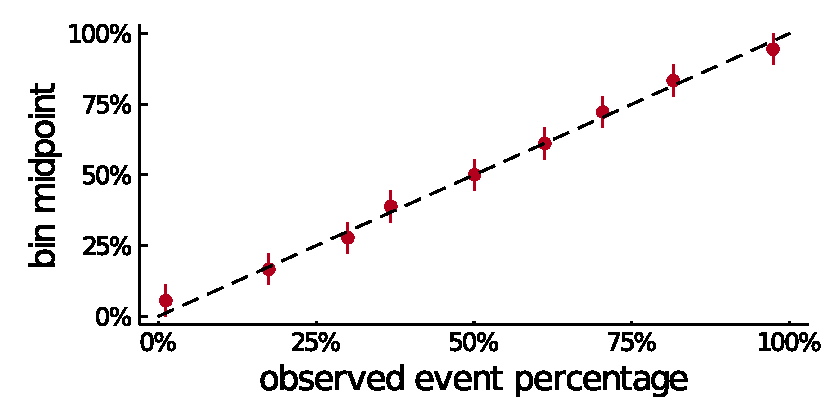
\includegraphics[width=1.0\linewidth]{plots/phylogeny_calibration.pdf}  
  \caption{Calibration plot for the HBV core protein.}
  \label{fig:calibration}
\end{figure}

%However, comparing against real-world data is not straight forward when identifying HLA-associated mutations, because if a tool identifies an HLA-associated mutation which is not yet documented, this could be either because it is a false positive, or a yet unknown HLA-associated mutation that has not been documented before. 
%Also, viewing every non-identified HLA-associated mutation that is listed in the literature as a false negative is not correct either, because documented escape mutations do not necessarily have to show in each sequence alignment.
%A third issue when comparing models is that HLA-associated mutations are not necessarily binary, so the true positive / false negative framework does not work as well.

%To circumvent these issues and still compare against real-world data, we chose the following strategy:
%For each model, all evaluated replacements are ranked by decreasing confidence of being an HLA associated mutation. That is, for Bayesian models we calculate the probability of the corresponding regression coefficient exceeding zero \(P(\beta_{HLA} > 0)\), for Fisher's exact test we sort HLA allele - replacement pairs by increasing p-values and for the Phylogenetic Dependency Network, we rank the associations by increasing q-values.
%Then, a list of known epitopes is used to create a plot of the cumulative number of replacements inside the boundary of a known epitope vs. the corresponding rank. The underlying assumption for this kind of model check is that we expect to see an enrichment of replacements that lie inside the region of known epitopes and that this enrichment is stronger for better performing models.

The predictions of all tested models are strongly enriched in epitopes over baselines, irrespective of dataset (Fig.~\ref{fig:comparison} for HBe protein and Supplementary Figures ...-... for other datasets). For the best ranked HAMs, Fisher's exact test performs about as well as the HAMdetector backbone logistic regression model (model~1 in Fig.~\ref{fig:comparison}). Each of the following three model stages of HAMdetector increases HAM enrichment further, independently of the dataset.
The horseshoe prior alone (model~2) is a drastic improvement over model~1, even though it does not include any external information. The logistic regression model with horseshoe prior works roughly as well as the Phylogenetic Dependency Network \cite{Carlson2008}, which includes much more information. Note that the line for the Phylogenetic Dependency Network is shorter because it only outputs associations with a q-value lower than 0.2 by default. Model~3 with its additional inclusion of phylogeny has higher enrichment than model~2, and finally, the full model~4 with the inclusion of epitope prediction leads to a further improvement. Note that model~4 only uses epitope \textit{prediction} software and does not use any information of experimentally confirmed epitopes. These are here only used for model evaluation.

\begin{figure}
  \centering
  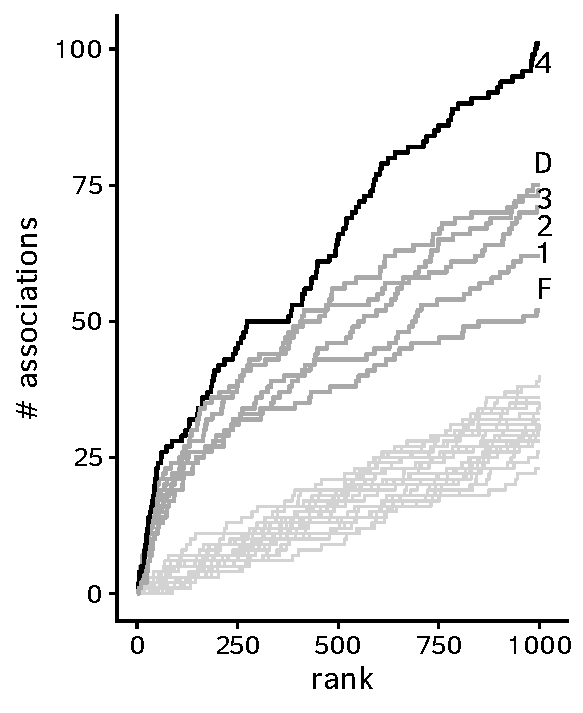
\includegraphics[width=0.8\linewidth]{plots/HBe.pdf}
  \caption{HAM enrichment plot for HBe protein: number $N_e$ of associations inside the boundary of known epitopes vs.\ rank $r$. D: Phylogenetic Dependency Network; F: Fisher's exact test; 1: simple logistic regression model with broad Student-t priors; 2: logistic regression model with horseshoe prior; 3: logistic regression model with horseshoe prior and phylogeny; 4: full model with epitope prediction. Unannotated gray lines at the bottom of the graph are HAM enrichment curves for random permutations of the list of HLA allele - replacement pairs and act as baselines.}
  \label{fig:comparison}
\end{figure}

The Bayesian approach lends itself to addition of prior knowledge, and it is not too surprising that exploiting this feature to incorporate information from phylogeny or epitope prediction improves HAM detection. It may be more surprising that the sparsifying horseshoe prior has such an impact. However, this is in principle the same mechanism as for the other information components: it is known that HAMs are sparse per HLA allele, and therefore supplying this information to the inference improves predictions. Figure~\ref{fig:horseshoe-comparison} illustrates the effect of the sparsifying prior with a concrete example, the replacement 11D in HIV integrase (Arevir dataset). There is no evidence for an association of HLA-A*01 with this replacement, whereas for HLA-B*44 the data is consistent with a strong association.  The horseshoe prior has the effect of shrinking towards 0 specifically those regression coefficients with weak evidence of an association (A*01 in Fig.~\ref{fig:horseshoe-comparison}). This reduces the standard error for the remaining coefficients, leading in our example to narrowed histogram for the association with B*44 in the model with horseshoe prior.

\begin{figure}
  \centering
  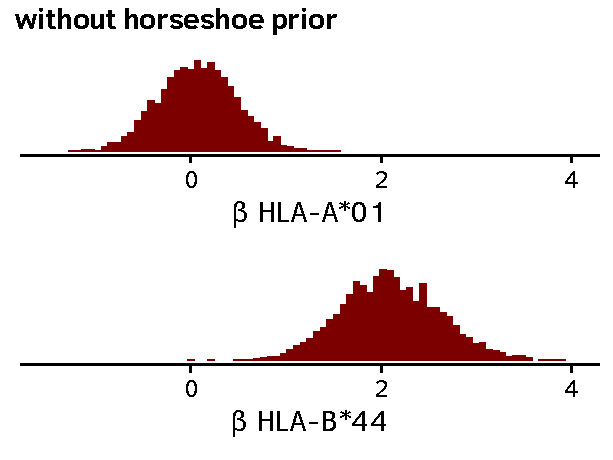
\includegraphics[width=0.8\linewidth]{plots/without_horseshoe.pdf}
  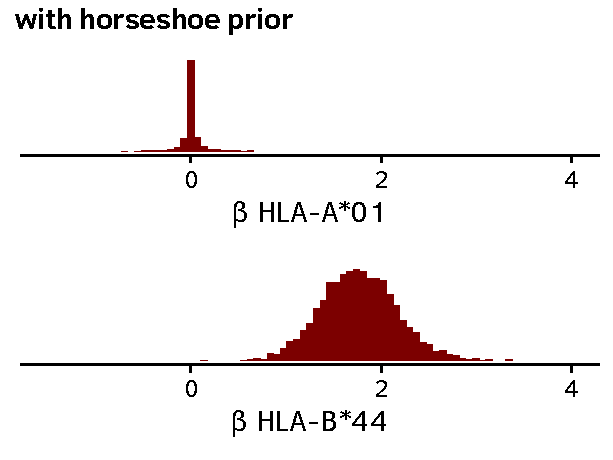
\includegraphics[width=0.8\linewidth]{plots/with_horseshoe.pdf}
  \caption{Marginal posterior distributions of regression coefficients for the association of replacement 11D of the HIV integrase with HLA alleles A*01 and B*44. Top half: inferred with logistic regression model, bottom half: inferred with logistic regression with sparsifying horseshoe prior.}
  \label{fig:horseshoe-comparison}
\end{figure}


\subsection{Leave-one-out cross-validation}

To quantify the ability of the four different model stages of HAMdetector to generalize to unseen cases, we computed the ELPD with Pareto-smoothed leave-one-out cross-validation. Table \ref{loo} shows results for the HBe protein of the HBV dataset in terms of ELPD changes with each new model stage. Each new model stage adds ELPD, i.e.\ is better at generalizing than the simpler model stages.

\begin{table}
  \renewcommand{\arraystretch}{1.3}
  \centering
  \caption{ELPD changes as HAMdetector components are added. Data computed for HBe protein of the HBV dataset. All differences in ELPD are larger than several times the estimated standard error (column \(\text{se}_\text{diff}\)), indicating that models that include more information have better predictive performance.}
  \vspace{0.5cm}
  \begin{tabular}{l|r|rll}
  \multicolumn{1}{l|}{} & \multicolumn{1}{c|}{\(\text{ELPD}_\text{diff}\)} & \multicolumn{1}{c}{\(\text{se}_\text{diff}\)} &  &  \\ \cline{1-3}
  logistic regression (baseline) & 0.0  & 0.0 &  &  \\
  + horseshoe prior     & 949.8  & 65.2 &  &  \\
  + phylogeny & 4440.9 & 94.4 &  &  \\
  + epitope prediction & 63.1   & 18.9 &  & 
  \end{tabular}
  \label{loo}
\end{table}


The model with horseshoe prior alone already has a much higher ELPD than the standard logistic regression model, even though it does not use any specific external data. This is because including the sparsity assumption allows the model to better separate signal from noise and the uncertainty of the close-to-zero coefficients does not propagate into uncertainty of predictions.

Including phylogeny further improves model performance a lot, as the assumption of independent and identically distributed data is replaced with specific information from the shared phylogenetic history.

While addition of sparsity and phylogeny has an effect on all replacements and samples, epitope prediction only influences those replacements that are restricted by a given HLA allele and only those samples that are annotated with the allele. Therefore, inclusion of epitope prediction does not improve ELPD as much as inclusion of phylogeny and the sparsity assumption. However, inclusion of epitope prediction is highly useful for determining which HLA alleles are associated with a replacement, as shown in the previous section.

\subsection{HAMs in HDV as test case}
The Hepatitis D Virus (HDV) dataset \citep{Karimzadeh2019} is an excellent test case: we have (1) a set of paired HDV sequences and patient HLA alleles, (2) HAM predictions by Fisher's exact test as implemented in SeqFeatR \citep{Budeus2016}, and (3) experimental tests of the predicted HAMs for immune escape activity (IFN-\(\gamma\) production assays, \citet{Karimzadeh2019}). This allows us to see whether HAMdetector decreases the false positive rate in comparison to the simpler Fisher's exact test, and we can make \emph{bona fide} predictions on previously undetected HAMs.
We have 15 HAMs predicted in HDV by Fisher's exact test at significance level $5\times 10^{-3}$ (Table~\ref{tab:false-positives}) as published \citep{Karimzadeh2019}. The corresponding p-values  have no clear relation to experimental confirmation, i.e.\ p-values for confirmed HAMs are not generally lower than those of non-confirmed ones.

For HAMdetector, we use in Table~\ref{tab:false-positives} the posterior probability of a positive regression coefficient ($P(\beta_{jk}>0)$ as measure for the confidence in having detected a HAM. HAMs with strong support have a posterior probability close to 1, associations with no support a probability close to 0.5 (corresponding to a regression coefficient centered around 0). The five predicted HAMs with top posterior probabilities (all $\ge 0.90$) have all been experimentally confirmed. There is only one outlier with posterior probability 0.75 (P89T and B*37).

HAMdetector strongly supports 15 replacement - allele pairs that have previously not been identified (question marks in last column of Table~\ref{tab:false-positives}). All of them have association probabilities of 0.90 or higher, while their p-values from Fisher's exact test exceed the significance level of $5\times 10^{-3}$ used in~\citet{Karimzadeh2019}. Given the superior performance of HAMdetector on the experimentally tested HAMs, these 15 bona fide predictions suggest that most true HAMs may still to be discovered. A striking example is K43R - A*02 with a p-value of 0.22 in Fisher's exact test but a HAM-probability of 0.90 and location inside an A*02 restricted epitope. 

\begin{table}[h!]
  \caption{List of HAMs predicted by Fisher's exact test (FET). In the last column ``+'' and ``-'' mark experimentally confirmed or rejected HAMs, respectively; ``?'' below the horizontal line indicate untested bona fide predictions. ``post.prob.'' are posterior probabilities for positive associations computed with HAMdetector.}
  \vspace{0.5cm}
  \begin{tabular}{c|c|c|c|c}
  replacement & allele  & p-value (FET) & post.~prob. & confirmed \\
  \hline
  S170N       & B*15 & $3\cdot10^{-8}$      & 0.99                                & +                        \\
  D101E       & B*37 & 0.0002                        & 0.96                                & +                        \\
  R105K       & B*27 & 0.0011                        & 0.93                                & +                        \\
  R139K       & B*41 & 0.0034                        & 0.92                                & +                        \\
  E47D        & B*18 & 0.0027                        & 0.90                                & +                        \\
  D33E        & B*13 & 0.0001                        & 0.86                                & -                        \\
  T134A       & A*68 & 0.0045                        & 0.82                                & -                        \\
  K43R        & B*13 & 0.0021                        & 0.77                                & -                        \\
  P89T        & B*37 & 0.0011                        & 0.75                                & +                        \\
  D47E        & A*30 & 0.0010                        & 0.76                                & -                        \\
  K113R       & B*13 & 0.0043                        & 0.76                                & -                        \\
  A107T       & B*14 & 0.0028                        & 0.70                                & -                        \\
  P49L        & A*30 & 0.0031                        & 0.63                                & -                        \\
  Q100L       & B*13 & 0.0018                        & 0.60                                & -                        \\
  D96E        & B*13 & 0.0035                        & 0.51                                & -  \\\hline
  E46D & A*02 & 0.0054 & 0.97 & ? \\
  V81I & A*68 & 0.0073 & 0.97 & ? \\
  K113N & B*08 & 0.0063 & 0.96 & ? \\
  A71T & B*41 & 0.0065 & 0.96 & ? \\
  L188I & A*68 & 0.0632 & 0.94 & ? \\
  T95S & A*01 & 0.0285 & 0.93 & ? \\
  D33E & A*03 & 0.0226 & 0.93 & ? \\
  P49L & B*13 & 0.0035 & 0.92 & ? \\
  A74S & A*68 & 0.0123 & 0.91 & ? \\
  E29D & B*44 & 0.0559 & 0.91 & ? \\
  D46E & B*57 & 0.0190 & 0.91 & ? \\
  R88K & A*68 & 0.0123 & 0.91 & ? \\
  T149P & B*52 & 0.0281 & 0.91 & ? \\
  K43R & A*02 & 0.2158 & 0.90 & ? \\
  N22S & B*08 & 0.0405 & 0.90 & ? \\
  \end{tabular}
  \label{tab:false-positives}
 \end{table}

 \subsection{Linkage disequilibrium}

 For three of the false positives proposed by Fisher's exact test (Table~\ref{tab:false-positives}), HAMdetector identifies associations with the same replacement but a different allele (P49L - B*13 instead of P49L - A*30; K43R - A*02 instead of K43R - B*13; and D33E - B*13 instead of D33E - A*03). One possible explanation for this observation is HLA linkage disequilibrium \hl{DaHo: and accordingly correlation between HLA alleles in the dataset due to random sampling variation. (Satz etwas opak.)} Indeed, out of the 12 times P49L is observed in sequences annotated with A*30, B*13 is also present in 5 of those cases (Spearman's rank correlation coefficient \(\rho = 0.5\)). A similar observation can be made for K43R and D33E, although the correlation between the respective alleles is much weaker.

\begin{figure}
  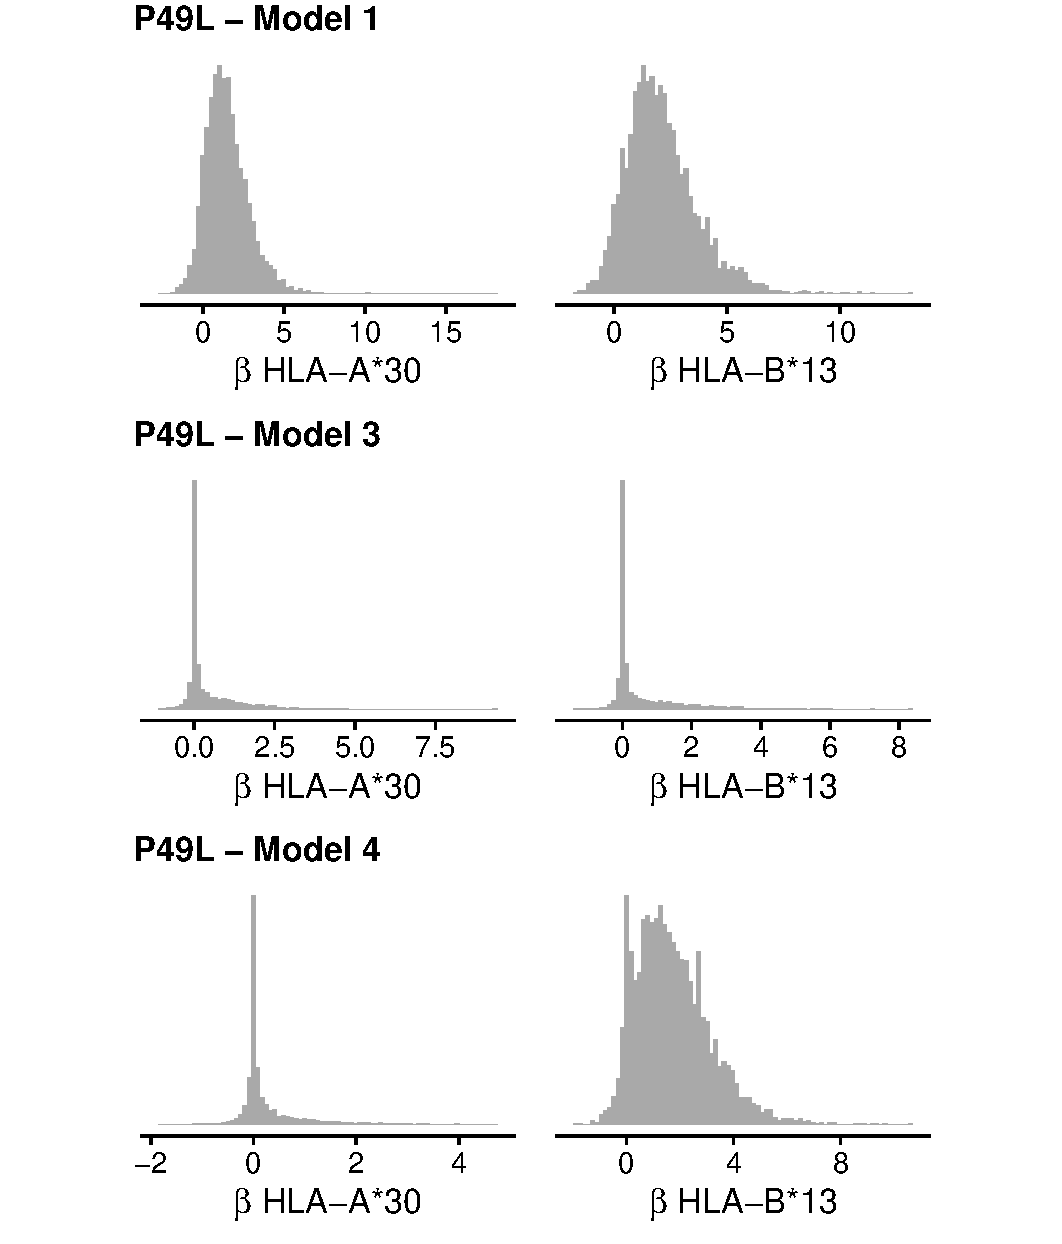
\includegraphics[width=1.1\linewidth]{plots/P49L_combined.pdf}
  \caption{Marginal posteriors for the regression coefficients of A*30 (left column) and B*13 (right column) for replacement P49L with different model stages (rows).}
  \label{fig:linkage}
\end{figure}

Figure~\ref{fig:linkage} shows regression coefficients of the HLA alleles A*30 and B*13 for replacement P49L. With the simplest logistic regression model (model~1), both A*30 and B*13 have medium evidence of being associated with replacement P49L. However, with phylogeny and sparsity-promoting prior (model~3) both regression coefficients shrink close to 0 -- the associations are not convincingly supported by the data. Using epitope prediction as additional source of information (model~4) allows to disentangle the association of the correlated alleles with P49L and identify B*13 as likely associated with P49L. The association between P49L and A*30 (predicted by Fisher's exact test) remains shrunk towards 0.  

\subsection{HAMs outside epitopes}
\label{sec:hams-outs-epit}

imperfect epitope / processing predictions

compensatory mutations

we expect HAMs outside epitopes - are there such HAMs?

Figure


\section{Discussion}

HAMdetector follows a general paradigm of Bayesian modelling, namely to map all information that is available about a system of interest onto a probabilistic model, and then to apply Bayesian inference to learn about probable parameter values of that model, e.g.\ about $\beta_{jk}$, the association of HLA $j$ with replacement $k$. The more relevant information we infuse into the model, the sharper the inference. As HAMdetector includes an unprecedented amount of relevant information, it is only natural that it outperforms other methods.

We have demonstrated that the logistic regression backbone is a platform that can be extended by model components that contribute new information. We have selected such modules guided by widely accepted knowledge, such as phylogeny or epitope location. However, even knowledge that is rarely stated explicitly may be helpful in inference, as in the case of sparsity of HLA associations. Since the included knowledge is generic for interactions of variable viruses with CTL immunity, HAMdetector performance does not depend on the virus.

Yet, HAMdetector is far from perfect. For instance the outlier in Table \ref{tab:false-positives} could point to missing information in HAMdetector. Another deficiency is that it currently works only with two-digit HLA alleles. We are currently exploring models for 4-digit HLA alleles that exploit partial pooling so that we can attenuate effects of the increased data fragmentation.

Another extension of our model would be to better account for phylogenetic uncertainty by using a Bayesian method to estimate a posterior distribution over possible tree topologies. The uncertainty over the tree topologies and the underlying parameters of the phylogenetic model would then propagate into uncertainty of the estimated probabilities \(P(y_{ik}=1|\Psi)\).

However, the good performance of the current version of HAMdetector makes it already a valuable tool for the study of interactions between viruses and T cell immunity.

%%%%%%%%%%%%%%%%%%%%%%%%%%%%%%%%%%%%%%%%%%%%%%%%%%%%%%%%%%%%%%%%%%%%%%%%%%%%%%%%%%%%% 
%
%     please remove the " % " symbol from \centerline{\includegraphics{fig01.eps}}
%     as it may ignore the figures.
%
%%%%%%%%%%%%%%%%%%%%%%%%%%%%%%%%%%%%%%%%%%%%%%%%%%%%%%%%%%%%%%%%%%%%%%%%%%%%%%%%%%%%%%






% \section{Conclusion}



%\section*{Acknowledgements}
% \FloatBarrier
\section*{Funding}

This work has been supported by Deutsche Forschungsgemeinschaft (grant HO 1582/10-1).\vspace*{-12pt}

\bibliographystyle{natbib}
%\bibliographystyle{achemnat}
%\bibliographystyle{plainnat}
%\bibliographystyle{abbrv}
%\bibliographystyle{bioinformatics}
%
%\bibliographystyle{plain}
%
\bibliography{references}
\end{document}
